Uma rede de sensores sem fio (RSSF) é um conjunto de dispositivos formando uma rede de comunicação \textit{ad-hoc}. Cada
sensor tem a capacidade de monitorar diversas propriedades físicas, como intensidade luminosa, temperatura, aceleração,
entre outras. Através de troca de mensagens, esses dispositivos podem agregar todas essas informações para detectar um evento
importante no local, como um incêndio. Essa conclusão é então encaminhada para um nó com maior capacidade computacional,
conhecido como estação base. Este nó pode decidir uma ação a ser tomada, ou enviar a informação pela Internet.

\begin{figure}
\centering
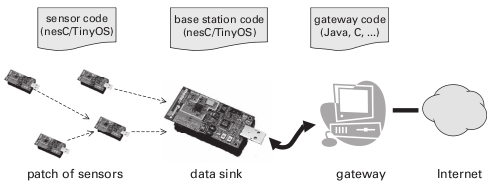
\includegraphics[scale=0.7]{images/sensores-e-topologia.png}
\caption{Rede de sensores sem fio}
\end{figure}

Estes sensores são desenvolvidos para monitoriar ambientes de difícil acesso, portanto, devem ser pequenos e utilizar
comunicação sem fio para facilitar a instalação no ambiente e minimizar o custo financeiro. Para evitar manutenções
frequêntes, eles também devem consumir pouca energia. Devido a estas características, o hardware destes dispositivos 
tende a ter recursos computacionais limitados. Ao invés de utilizar CPUs, são usados microcontroladores de 8 ou 16 bits, 
normalmente, com baixas frequências de relógio. Para armazenar o código da aplicação é utilizada uma pequena memória flash, 
da ordem de 100kB, e para as variáveis existe uma memória RAM, da ordem de 10kB. Os circuitos de rádio também têm uma 
capacidade reduzida de transferência, da ordem de kilobytes por segundos~\cite{LevisGay/09}.
Aliado ao hardware, o software também deve ser voltado para o baixo consumo de energia e de memória. Detalhes serão
vistos na próxima seção. 

Uma RSSF é usada para monitorar ambientes de difícil acesso, onde uma rede cabeada seria inviável ou custosa.
Alguns exemplos reais do uso de RSSF são: monitoramento da ponte Golden Gate em São Francisco, e dos vulcões Reventador e 
Tungurahua no Equador~\cite{LevisGay/09}. 

